
%%%%%%%%%%%%%%%%%%%%%%%%%%%%%%%%%%%%%%%%%%%%%%%%%%%%%%%%%%%%%%%%%%

\newpage
\chapter{Methodology}


\section{Introduction}
ElderCare Connect is a Progressive Web App (PWA) designed to improve the safety, health monitoring, and social engagement of elderly individuals living alone. The app enables real-time health tracking, emergency alerts, and fosters social connections to combat loneliness among the elderly. With features like integration with Google Fit, emergency call APIs, and push notifications, the app aims to offer a comprehensive solution for elderly care.  
The app is available across multiple devices (smartphones, tablets, and desktops) without requiring installation, ensuring accessibility for elderly users who may have limited technical knowledge. Through this project, we aim to create a solution that enhances the well-being of elderly people, provides peace of mind to their families, and ensures prompt emergency response when necessary\cite{eldercare_solutions}.

\section{Importance of Implementation}
The implementation phase is the most critical in turning the conceptual design of ElderCare Connect into a fully functioning app. It is at this stage where the app's core features are developed, tested, and optimized for real-world use. Effective implementation ensures that the app is functional, secure, and scalable, fulfilling its purpose of supporting elderly individuals.  
This phase involves integrating various technologies and services, such as health tracking with wearable devices, push notifications for emergencies, and secure authentication with JWT. It also includes rigorous system testing to detect and fix any issues before deployment. The implementation of these features directly impacts user experience, reliability, and the app's ability to meet its intended goals\cite{pwa_development}.

\section{Implementation Methodology}

The development of ElderCare Connect followed an Agile methodology, which allowed for iterative development and continuous feedback from stakeholders\cite{agile_manifesto}. The project was broken down into smaller, manageable tasks that were completed in sprints, ensuring that each feature was developed, tested, and integrated step by step\cite{scrum_guide}. This approach allowed the team to make improvements based on real-time feedback and user testing.

\begin{itemize}
    \item \textbf{Sprint 1:} Requirements gathering and setup of the development environment.
    \item \textbf{Sprint 2:} Frontend development (UI/UX design, layout creation using Next.js and Tailwind CSS)\cite{nextjs_docs}.
    \item \textbf{Sprint 3:} Backend development (API setup with Node.js and Express, Firebase integration for real-time notifications)\cite{nextjs_docs}.
    \item \textbf{Sprint 4:} Integration of real-time health monitoring (Google Fit)\cite{google_fit}.
    \item \textbf{Sprint 5:} Security implementation (JWT authentication, SSL encryption)\cite{jwt_handbook}.
    \item \textbf{Sprint 6:} Testing, deployment, and final refinements based on user feedback\cite{firebase_docs}.
\end{itemize}

\section{Implementation Environment}

The implementation environment for ElderCare Connect consists of various tools and technologies that support both frontend and backend development.

\subsection*{Frontend:}
\begin{itemize}
    \item \textbf{Next.js:} Chosen for its ability to build server-side rendered React applications, making the app more SEO-friendly and performant\cite{nextjs_docs}.
    \item \textbf{Tailwind CSS:} A utility-first CSS framework that enabled rapid design implementation\cite{tailwind_docs}.
\end{itemize}

\subsection*{Backend:}
\begin{itemize}
    \item \textbf{Node.js:} The backend is built with Node.js due to its non-blocking, event-driven architecture, making it ideal for real-time data handling\cite{nodejs_docs}.
    \item \textbf{Express.js:} A web application framework for Node.js, used to handle routing and middleware for API requests\cite{express_docs}.
    \item \textbf{MongoDB/Firebase:} MongoDB is used for storing user data and health records, while Firebase handles real-time notifications and authentication\cite{mongodb_docs}.
\end{itemize}

\subsection*{Other Tools:}
\begin{itemize}
    \item \textbf{Git:} Version control system for team collaboration\cite{git_docs}.
    \item \textbf{Postman:} Used for API testing during development\cite{postman_docs}.
    \item \textbf{Firebase Cloud Messaging (FCM):} For sending push notifications, emergency alerts, and real-time medication reminders\cite{firebase_fcm}.
    \item \textbf{Jest:} A testing framework used to ensure that the backend APIs function as expected\cite{jest_docs}.
\end{itemize}

\section{Tools Used}

\subsection*{Frontend:}
\begin{itemize}
    \item \textbf{Next.js:} Framework for building React-based web applications.
    \item \textbf{Tailwind CSS:} Used for creating responsive and modern designs.
    \item \textbf{Figma:} Design tool for UI/UX wireframing and prototyping.
\end{itemize}

\subsection*{Backend:}
\begin{itemize}
    \item \textbf{Node.js:} JavaScript runtime for the server-side environment.
    \item \textbf{Express.js:} Web framework for building APIs.
    \item \textbf{MongoDB/Firebase:} Database management (MongoDB for storing data, Firebase for real-time notifications and authentication).
    \item \textbf{JWT:} JSON Web Token used for secure authentication.
\end{itemize}

\subsection*{Testing:}
\begin{itemize}
    \item \textbf{Jest:} For unit and integration testing.
    \item \textbf{Postman:} For testing the backend API endpoints.
\end{itemize}

\subsection*{Version Control:}
\begin{itemize}
    \item \textbf{Git:} Used for source code management and version control, with GitHub for collaboration.
\end{itemize}

\section{\System Testing}

System testing was carried out to ensure that the ElderCare Connect app functions as expected under various conditions. The testing process included:

\begin{itemize}
    \item \textbf{Unit Testing:} Testing individual components like the login system, emergency alerts, and API endpoints using Jest\cite{jest_docs}.
    \item \textbf{Integration Testing:} Ensuring that components such as the frontend, backend, and Firebase service work seamlessly together\cite{firebase_testing}.
    \item \textbf{User Acceptance Testing (UAT):} Involving actual users to test the app’s usability and gather feedback on its features and design\cite{uat_testing}.
    \item \textbf{Performance Testing:} Checking the app's ability to handle real-time notifications and large datasets without delays\cite{performance_testing}.
    \item \textbf{Security Testing:} Ensuring that data, especially health-related data, is securely transmitted using SSL encryption, and verifying the robustness of JWT-based authentication\cite{security_testing}\cite{jwt_security}.
\end{itemize}

\section{Technical Stack}

\begin{itemize}
    \item \textbf{Frontend:} Next.js, Tailwind CSS
    \item \textbf{Backend:} Node.js, Express.js
    \item \textbf{Database:} MongoDB, Firebase
    \item \textbf{Real-Time Services:} Firebase Cloud Messaging (FCM), WebSockets
    \item \textbf{Authentication:} JWT (JSON Web Token)
    \item \textbf{Security:} SSL encryption
    \item \textbf{Testing Tools:} Jest, Postman
    \item \textbf{Version Control:} Git, GitHub
    \item \textbf{Deployment:} Firebase Hosting
\end{itemize}

\section{Gantt Chart}

\begin{figure}[htbp]
  \centering
  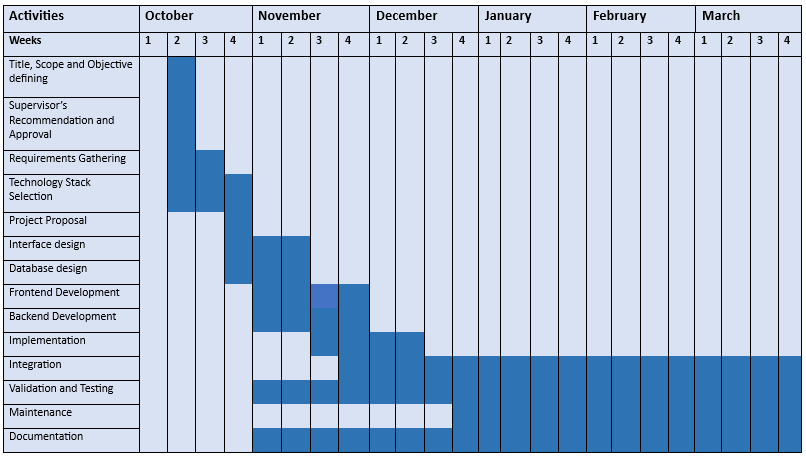
\includegraphics[width=6.4in]{ganttchart.PNG}
  \caption{Timeline}
  \label{fig:ganttchart}
\end{figure}



 


